\section{Kiến trúc hệ thống}\label{sec:03-system-architecture}
\subsection{Tổng thể các thành phần}
Hệ thống gồm ứng dụng Flutter tạo thông tin cầu cứu, backend FastAPI tiếp nhận và lưu trữ, lõi \texttt{rescue\_core} phân cụm/xếp hạng, và dashboard web phục vụ điều phối. SQLite giữ trạng thái bền vững tại backend; ảnh lưu ở thư mục uploads. Mô hình ảnh và mô hình khẩn cấp có cấu trúc thuộc phần tạo đặc trưng tại ứng dụng. Các notebook nghiên cứu là một đường đánh giá riêng, không chạy bên trong dashboard.

\begin{figure}[htbp]
\centering
\begin{tikzpicture}[node distance=9mm,>=Stealth,
 box/.style={draw,rounded corners,align=center,text width=49mm,minimum height=15mm,font=\small},
 store/.style={box,fill=blue!7}]
\node[box] (user) {Người gửi\\SOS, mô tả, ảnh, GPS};
\node[store,below=of user] (app) {Flutter\\AI và outbox cục bộ};
\node[box,right=13mm of app] (backend) {FastAPI\\kiểm tra hợp đồng và ACK};
\node[store,below=of backend] (db) {SQLite và ảnh\\báo cáo, dedup, nhật ký};
\node[box,below=of app] (core) {rescue\_core\\đồ thị, cụm, điểm ưu tiên};
\node[box,below=of core] (dashboard) {Dashboard điều phối\\bản đồ, đội, trạng thái};
\draw[->] (user)--(app);
\draw[<->] (app)--node[above,font=\scriptsize,align=center]{HTTP\\ACK}(backend);
\draw[<->] (backend)--(db);
\draw[->] (db)--(core);
\draw[->] (core)--(dashboard);
\draw[->] (dashboard.east)-|(db.south);
\end{tikzpicture}
\caption{Kiến trúc chức năng của hệ thống demo đang có trong repo}
\label{fig:system-architecture}
\end{figure}

Dữ liệu từ điện thoại và dữ liệu nạp demo dùng chung API/lưu trữ, nhưng nguồn mô phỏng được gắn nhãn để tránh nhầm với yêu cầu thực tế. Backend nạp run\_001 khi volume trống trong cấu hình demo; đây là 316 báo cáo bán tổng hợp. Việc dashboard có dữ liệu và nhiều cụm sau seed chỉ chứng minh đường tích hợp hoạt động với dữ liệu đó.

\subsection{Phân lớp ứng dụng Flutter}
Mã đang được nối từ \texttt{main.dart} phân thành data, domain và presentation. Data chứa datasource cục bộ/từ xa và repository implementation. Domain chứa entity, repository interface, use case và các chính sách thuần. Presentation chứa controller, màn hình và widget. Phân lớp cho phép kiểm tra chính sách gửi, hash và trạng thái mà không cần plugin thiết bị.

Datasource suy luận dùng conditional export để chọn bản native/web. ONNX được gọi qua runtime Dart ở nền tảng hỗ trợ; ExecuTorch Android được gọi qua MethodChannel \texttt{rescue/executorch}. MethodChannel \texttt{rescue/sms} nối tới SMS Android. Bản web không có đường suy luận ảnh native hoặc gửi SMS; nó phù hợp kiểm thử luồng giao diện, HTTP, offline/reconnect và điều phối.

Trong repo còn cây mã legacy ở các tệp như \RepoPath{controller.dart}, \RepoPath{home_screen.dart} và \texttt{services/}. Chúng không phải toàn bộ đường thực thi hiện tại từ \texttt{main.dart}. Phân tích báo cáo bám vào cây data/domain/presentation; lỗi analyze ở mã legacy được giữ như hạn chế kỹ thuật, không dùng để suy ra mọi luồng hiện tại không hoạt động.

\subsection{Lưu trữ cục bộ và hàng đợi}
Khi tạo báo cáo, ứng dụng ghi bản ghi và dữ liệu cần đồng bộ vào Hive. Outbox giữ message cùng định danh, hash, sequence và số lần thử. Repository điều phối gửi metadata/ảnh và chỉ xử lý hoàn tất khi phản hồi phù hợp. Nếu ảnh chưa gửi được, metadata hoặc bản ghi vẫn có thể tồn tại để tiếp tục lần sau.

Việc chọn chế độ gửi được thực hiện khi có ảnh và được xem xét lại khi hàng đợi gửi sau gián đoạn. Không nên dùng nguyên đánh giá mạng cũ cho một lần đồng bộ mới. Workmanager định kỳ khoảng 15 phút trên nền tảng hỗ trợ; controller còn kích hoạt đồng bộ theo trạng thái kết nối. Chu kỳ khai báo không bảo đảm hệ điều hành sẽ thực thi đúng thời điểm trong mọi điều kiện nền hoặc tiết kiệm pin.

Địa điểm báo cáo có thể null. Màn hình trung tâm cần có danh sách cho báo cáo thiếu vị trí ngoài bản đồ, bởi một bản ghi không xuất hiện trên bản đồ không có nghĩa không cần xử lý. Vị trí được nhập thủ công có nguồn \texttt{manual}; khi GPS thiết bị đến sau, hợp đồng quy định cách bổ sung/thay thế để giữ nguồn gốc.

\subsection{Hợp đồng truyền thông}
Hợp đồng phiên bản 1 được xác nhận bằng header \texttt{X-Message-Contract-Version}. Metadata truyền qua \texttt{POST /sync/messages}; ảnh qua \texttt{POST /api/reports} dạng multipart với phần JSON \texttt{meta}. Batch có tối đa 50 message và 256 KiB; mỗi message có phản hồi riêng để app biết message nào nhận, trùng hoặc bị từ chối.

Payload hash dùng SHA-256 của JSON chuẩn tắc RFC 8785 \citep{rfc8785}. Phần chuẩn tắc phải tạo cùng byte ở Dart và Python, nhất là biểu diễn số và thứ tự thuộc tính. Hash ở đây kiểm tra nội dung phù hợp định danh, không tự chứng minh danh tính người gửi hoặc sự thật của hiện trường.

Một request có thể mất ACK sau khi transaction thành công. Khi app gửi lại cùng message và hash, backend trả duplicate thay vì tạo thao tác mới. Nếu cùng message ID nhưng nội dung khác, trả \texttt{ID\_REUSED\_WITH\_DIFFERENT\_PAYLOAD}. Nếu cặp client/sequence bị tái sử dụng, trả \texttt{SEQUENCE\_REUSED}. Cơ chế này cho phép retry trong mạng gián đoạn mà không đánh đổi tính nhất quán.

\subsection{Lưu trữ backend}
SQLite giữ bảng \texttt{reports}, \texttt{messages\_dedup}, \texttt{report\_events}, \texttt{teams}, \texttt{operators}, \texttt{sessions} và \texttt{server\_meta}. Ảnh nằm ngoài CSDL; bản ghi lưu tên, URL, hash và kích thước. Bảng báo cáo giữ payload gốc để bảo toàn những trường nghiên cứu chưa có cột riêng.

\begin{figure}[htbp]
\centering
\begin{tikzpicture}[node distance=10mm,>=Stealth,
 box/.style={draw,align=center,text width=42mm,minimum height=16mm,font=\small}]
\node[box] (reports) {reports\\id, vị trí, status, payload};
\node[box,left=9mm of reports] (events) {report\_events\\report\_id, actor, thời gian};
\node[box,below=of reports] (teams) {teams\\đội được giao};
\node[box,below=of events] (ops) {operators / sessions\\tài khoản và phiên};
\node[box,below=of teams] (dedup) {messages\_dedup\\message, hash,\\client, sequence};
\draw[->] (events)--node[above,font=\footnotesize]{nhật ký}(reports);
\draw[->] (reports)--node[right,font=\scriptsize]{giao đội}(teams);
\draw[dashed,->] (ops)--node[left,font=\scriptsize]{actor}(events);
\draw[dashed,->] (dedup.east)--++(8mm,0)|-(reports.east);
\end{tikzpicture}
\caption{Quan hệ logic chính của lưu trữ; nét đứt biểu diễn liên hệ nghiệp vụ}
\label{fig:data-relations}
\end{figure}

Transaction theo từng message giúp lỗi của một phần batch không hủy các phần hợp lệ khác. Chế độ WAL cho phép dashboard đọc khi app ghi. \texttt{server\_meta} giữ sequence thay đổi, epoch và version đầu vào cụm. Migration bổ sung cột/bảng và chuẩn hóa trạng thái legacy khi khởi tạo, giữ dữ liệu hiện có.

Cùng report ID được gửi lại để bổ sung ảnh hoặc dữ liệu sau mất ACK được xử lý theo quy tắc gộp. Backend giữ ảnh đầu tiên, thời điểm nhận đầu và các trường đã có; số bằng không là dữ liệu hợp lệ, không xem như trường trống. \texttt{owner\_client\_id} tham gia kiểm tra quyền gộp. Quyền sở hữu dựa trên client ID giúp chống sửa chéo theo hợp đồng hiện tại, nhưng không tự thay thế xác thực danh tính người gửi.

\subsection{Dịch vụ phân cụm và hàng xem xét}
Adapter \texttt{to\_report\_v2} chuyển báo cáo lưu trữ sang tuple thuật toán. Nhãn ngập được ánh xạ \texttt{non\_flood}$\mapsto0$, \texttt{low}$\mapsto0{,}33$, \texttt{medium}$\mapsto0{,}66$, \texttt{high}$\mapsto1$. Nếu payload có \texttt{flood}, dùng trường này. Điểm khẩn cấp đọc \texttt{urgency} hoặc suy từ mô tả. $N$ hiện là số mắc kẹt cộng số bị thương; $V$ là số nhóm yếu thế được chọn khi không có trường trực tiếp.

Các ánh xạ trên là heuristic vận hành. Số nhóm không đồng nghĩa số người yếu thế; tổng mắc kẹt và bị thương có thể đếm trùng một người. Dữ liệu mô phỏng có trường trực tiếp không chịu đúng cùng sai số trích xuất như app. Vì vậy, benchmark lõi không thay thế kiểm định adapter trên báo cáo thực.

Báo cáo resolved/cancelled được loại khỏi cụm đang hoạt động. Cụm được tính lại khi version dữ liệu liên quan thay đổi; nếu một lần tính kéo dài, dịch vụ có cơ chế cập nhật nền. \texttt{clusterId} có thể đổi giữa lần chạy, còn \texttt{clusterKey} dùng ID nhỏ nhất trong cụm để hỗ trợ giữ lựa chọn trên giao diện. Khóa này cũng có thể đổi khi thành viên thay đổi; các thao tác điều phối cần xác nhận danh sách hiện tại.

\subsection{Dashboard và vòng phản hồi}
Dashboard là HTML, ES module và CSS phục vụ từ backend hoặc nginx. Leaflet được vendored để thư viện giao diện không cần CDN; lớp nền bản đồ có yêu cầu kết nối riêng tùy cấu hình nguồn tile. Giao diện polling báo cáo thay đổi và cụm mỗi 5 giây, dùng cursor/epoch và ETag để giảm tải so với tải lại toàn bộ.

Điều phối viên có thể lọc theo trạng thái/cụm, xem chi tiết, gán đội, ghi chú, cập nhật vị trí và chuyển trạng thái. API quản trị hỗ trợ quản lý tài khoản và sao lưu. Nhật ký \texttt{report\_events} ghi actor, nguồn và thời gian thao tác để theo dõi quá trình xử lý. App hỏi trạng thái báo cáo mỗi 15 giây và khi kết nối trở lại; đây là phản hồi định kỳ, không phải push tức thời.

\subsection{Ranh giới nghiên cứu và vận hành}
Luồng thuật toán được minh họa lại ở Hình~\ref{fig:research-pipeline}. Trường quan sát đi vào đồ thị, xếp hạng và scheduler; trường thiếu đi tới review; truth chỉ nối sau đầu ra. Hệ thống demo hiện tại cung cấp danh sách ưu tiên và thao tác điều phối do người dùng thực hiện. Scheduler tự động trong RQ3 là thành phần đánh giá nghiên cứu, không được đồng nhất với chức năng giao đội trên dashboard.
\begin{figure}[htbp]
\centering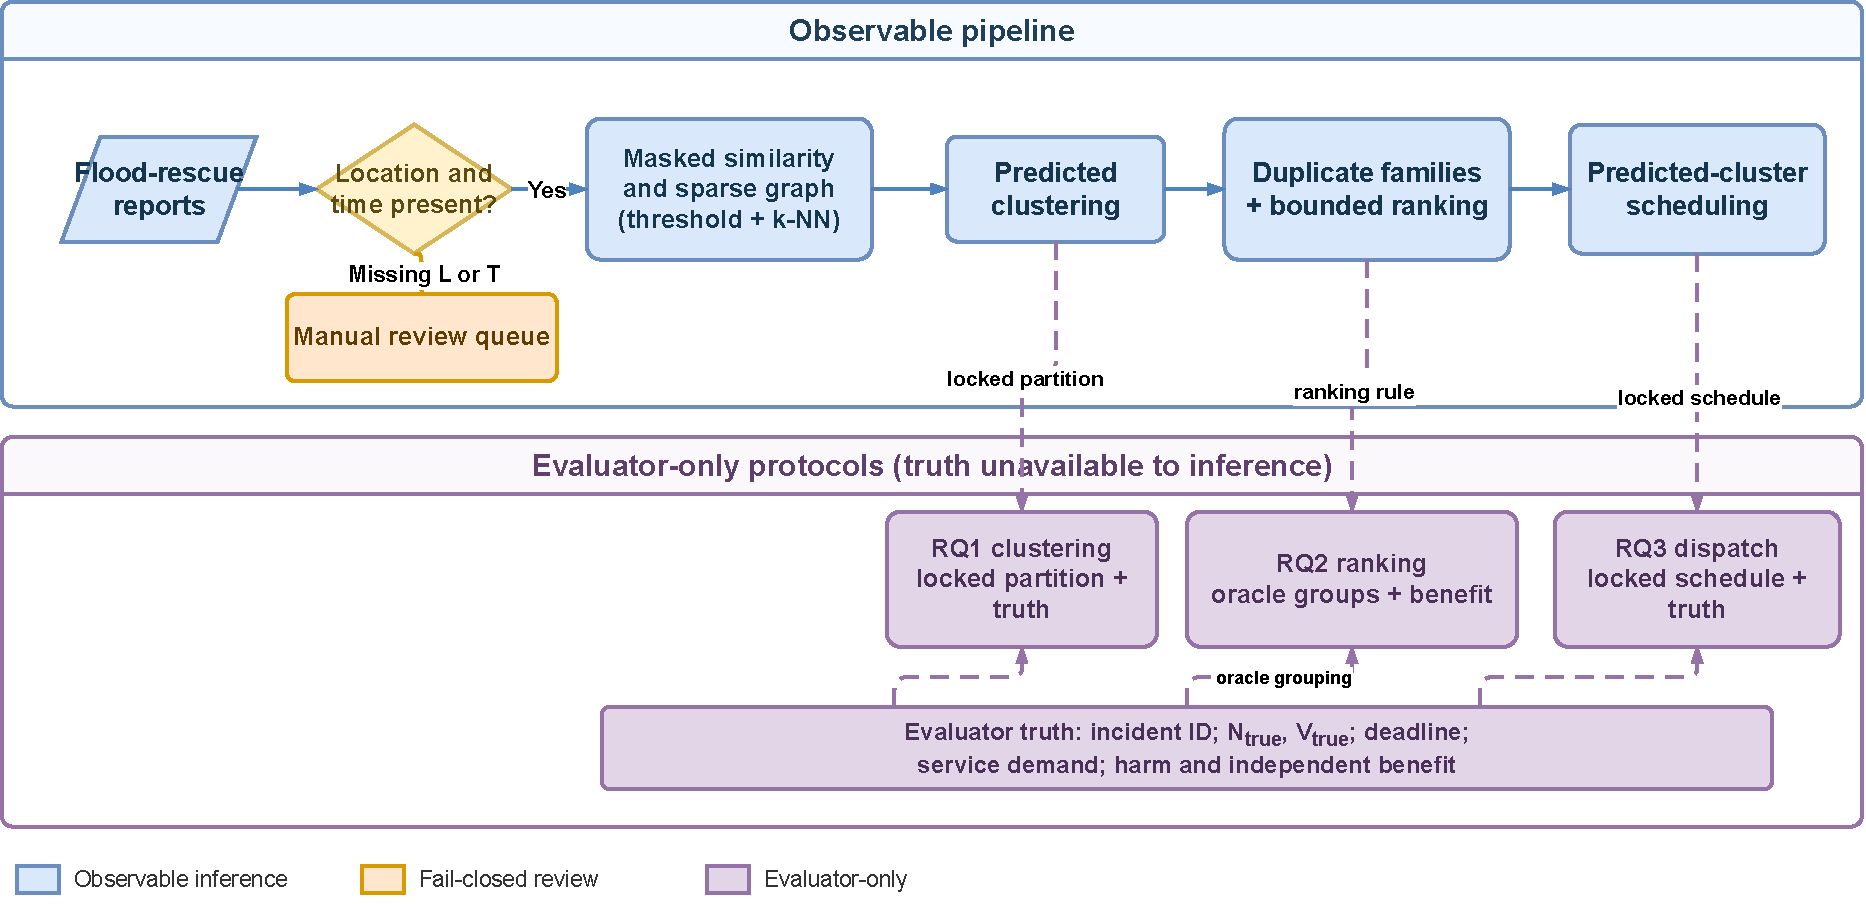
\includegraphics[width=\textwidth]{../paper/figures/pipeline_v2.pdf}
\caption{Ranh giới dữ liệu quan sát, hàng xem xét và evaluator của pipeline nghiên cứu}
\label{fig:research-pipeline}
\end{figure}
